\chapter{Seafloor Exploration Time Lapse}
\lhead{Seafloor Exploration Time Lapse}
\label{Appendix:SeafloorExplorationTimeLapse}

	The following sections provide the time lapse images from executing the informative path planning algorithms that generated the results in Section \ref{InformativeSeafloorExploration:ScottReef}. Sections \ref{Appendix:SeafloorExplorationTimeLapse:Single} and \ref{Appendix:SeafloorExplorationTimeLapse:Serial} provides the time lapse images corresponding to Section \ref{InformativeSeafloorExploration:ScottReef:SingleMission} and Section \ref{InformativeSeafloorExploration:ScottReef:SerialMission} respectively.
	
	\section{Single Mission Planning}
	\label{Appendix:SeafloorExplorationTimeLapse:Single}

			Figures \ref{Figure:OptimalPaths} show snapshots of the resulting path under LMDE and MCPIE acquisition respectively for single mission planning. Since in the end it is the prediction accuracy, instead of the model accuracy, that determines mapping and classification accuracy, the paths are layered onto the prediction information entropy (PIE) map for this visualisation. The snapshots are taken at 0.17 km (1\%), 16.67 km (50\%), and 33.33 km (100\%) into the journey.
				
			\begin{figure}[!htbp]
			\centering
			  \subfigure[LMDE Acquisition]{\label{Figure:OptimalPaths:LMDE} 
			  	\includegraphics[width = 0.32\linewidth]{Figures/informative_seafloor_exploration/lmde/mie_propose1.eps}
			  	\includegraphics[width = 0.32\linewidth]{Figures/informative_seafloor_exploration/lmde/mie_propose100.eps}
			  	\includegraphics[width = 0.32\linewidth]{Figures/informative_seafloor_exploration/lmde/mie_propose200.eps}}
			  \subfigure[MCPIE Acquisition]{\label{Figure:OptimalPaths:MCPIE}	
			  	\includegraphics[width = 0.32\linewidth]{Figures/informative_seafloor_exploration/mcpie/mie_propose1.eps}
			  	\includegraphics[width = 0.32\linewidth]{Figures/informative_seafloor_exploration/mcpie/mie_propose100.eps}
			  	\includegraphics[width = 0.32\linewidth]{Figures/informative_seafloor_exploration/mcpie/mie_propose200.eps}}
			\caption{Scott Reef: Exploration paths}
			\label{Figure:OptimalPaths}
			\end{figure}
			
			Under LMDE acquisition, as seen in Figure \ref{Figure:OptimalPaths:LMDE}, the AUV starts from the reef center, travels to the reef edge, returns from the reef edge to observe another inner region, and finally continues to map the reef edge. On the other hand, in Figure \ref{Figure:OptimalPaths:MCPIE}, the AUV simply travels to the reef edge and continues to observe the edges under MCPIE acquisition. As such, both methods focuses on the edges of the reef. However, LMDE acquisition did not neglect other regions while focusing on the reef edge, as it understands that too many observations at similar bathymetric signatures will introduce bias in the model.
			
			This difference is visible through the lower amount of prediction information entropy around the inner regions of the reef under LMDE acquisition compared to MCPIE acquisition, demonstrating better prediction accuracy. Interestingly, although MCPIE acquisition is the joint form of prediction information entropy, it is LMDE acquisition that achieves lower overall prediction information entropy. As discussed in Section \ref{InformativeSeafloorExploration:ComparisonMutualEntropyMeasures:EstimationAccuracy}, while MCPIE acquisition focuses on prediction variance, LMDE acquisition focuses on model variance which translate to both prediction variance and bias. Hence, in general, LMDE acquisition achieves better performance in the long run.

			\begin{figure}[!htbp]
			\centering
			  \subfigure[Initial Starting Positions]{\label{Figure:CompareLocations}	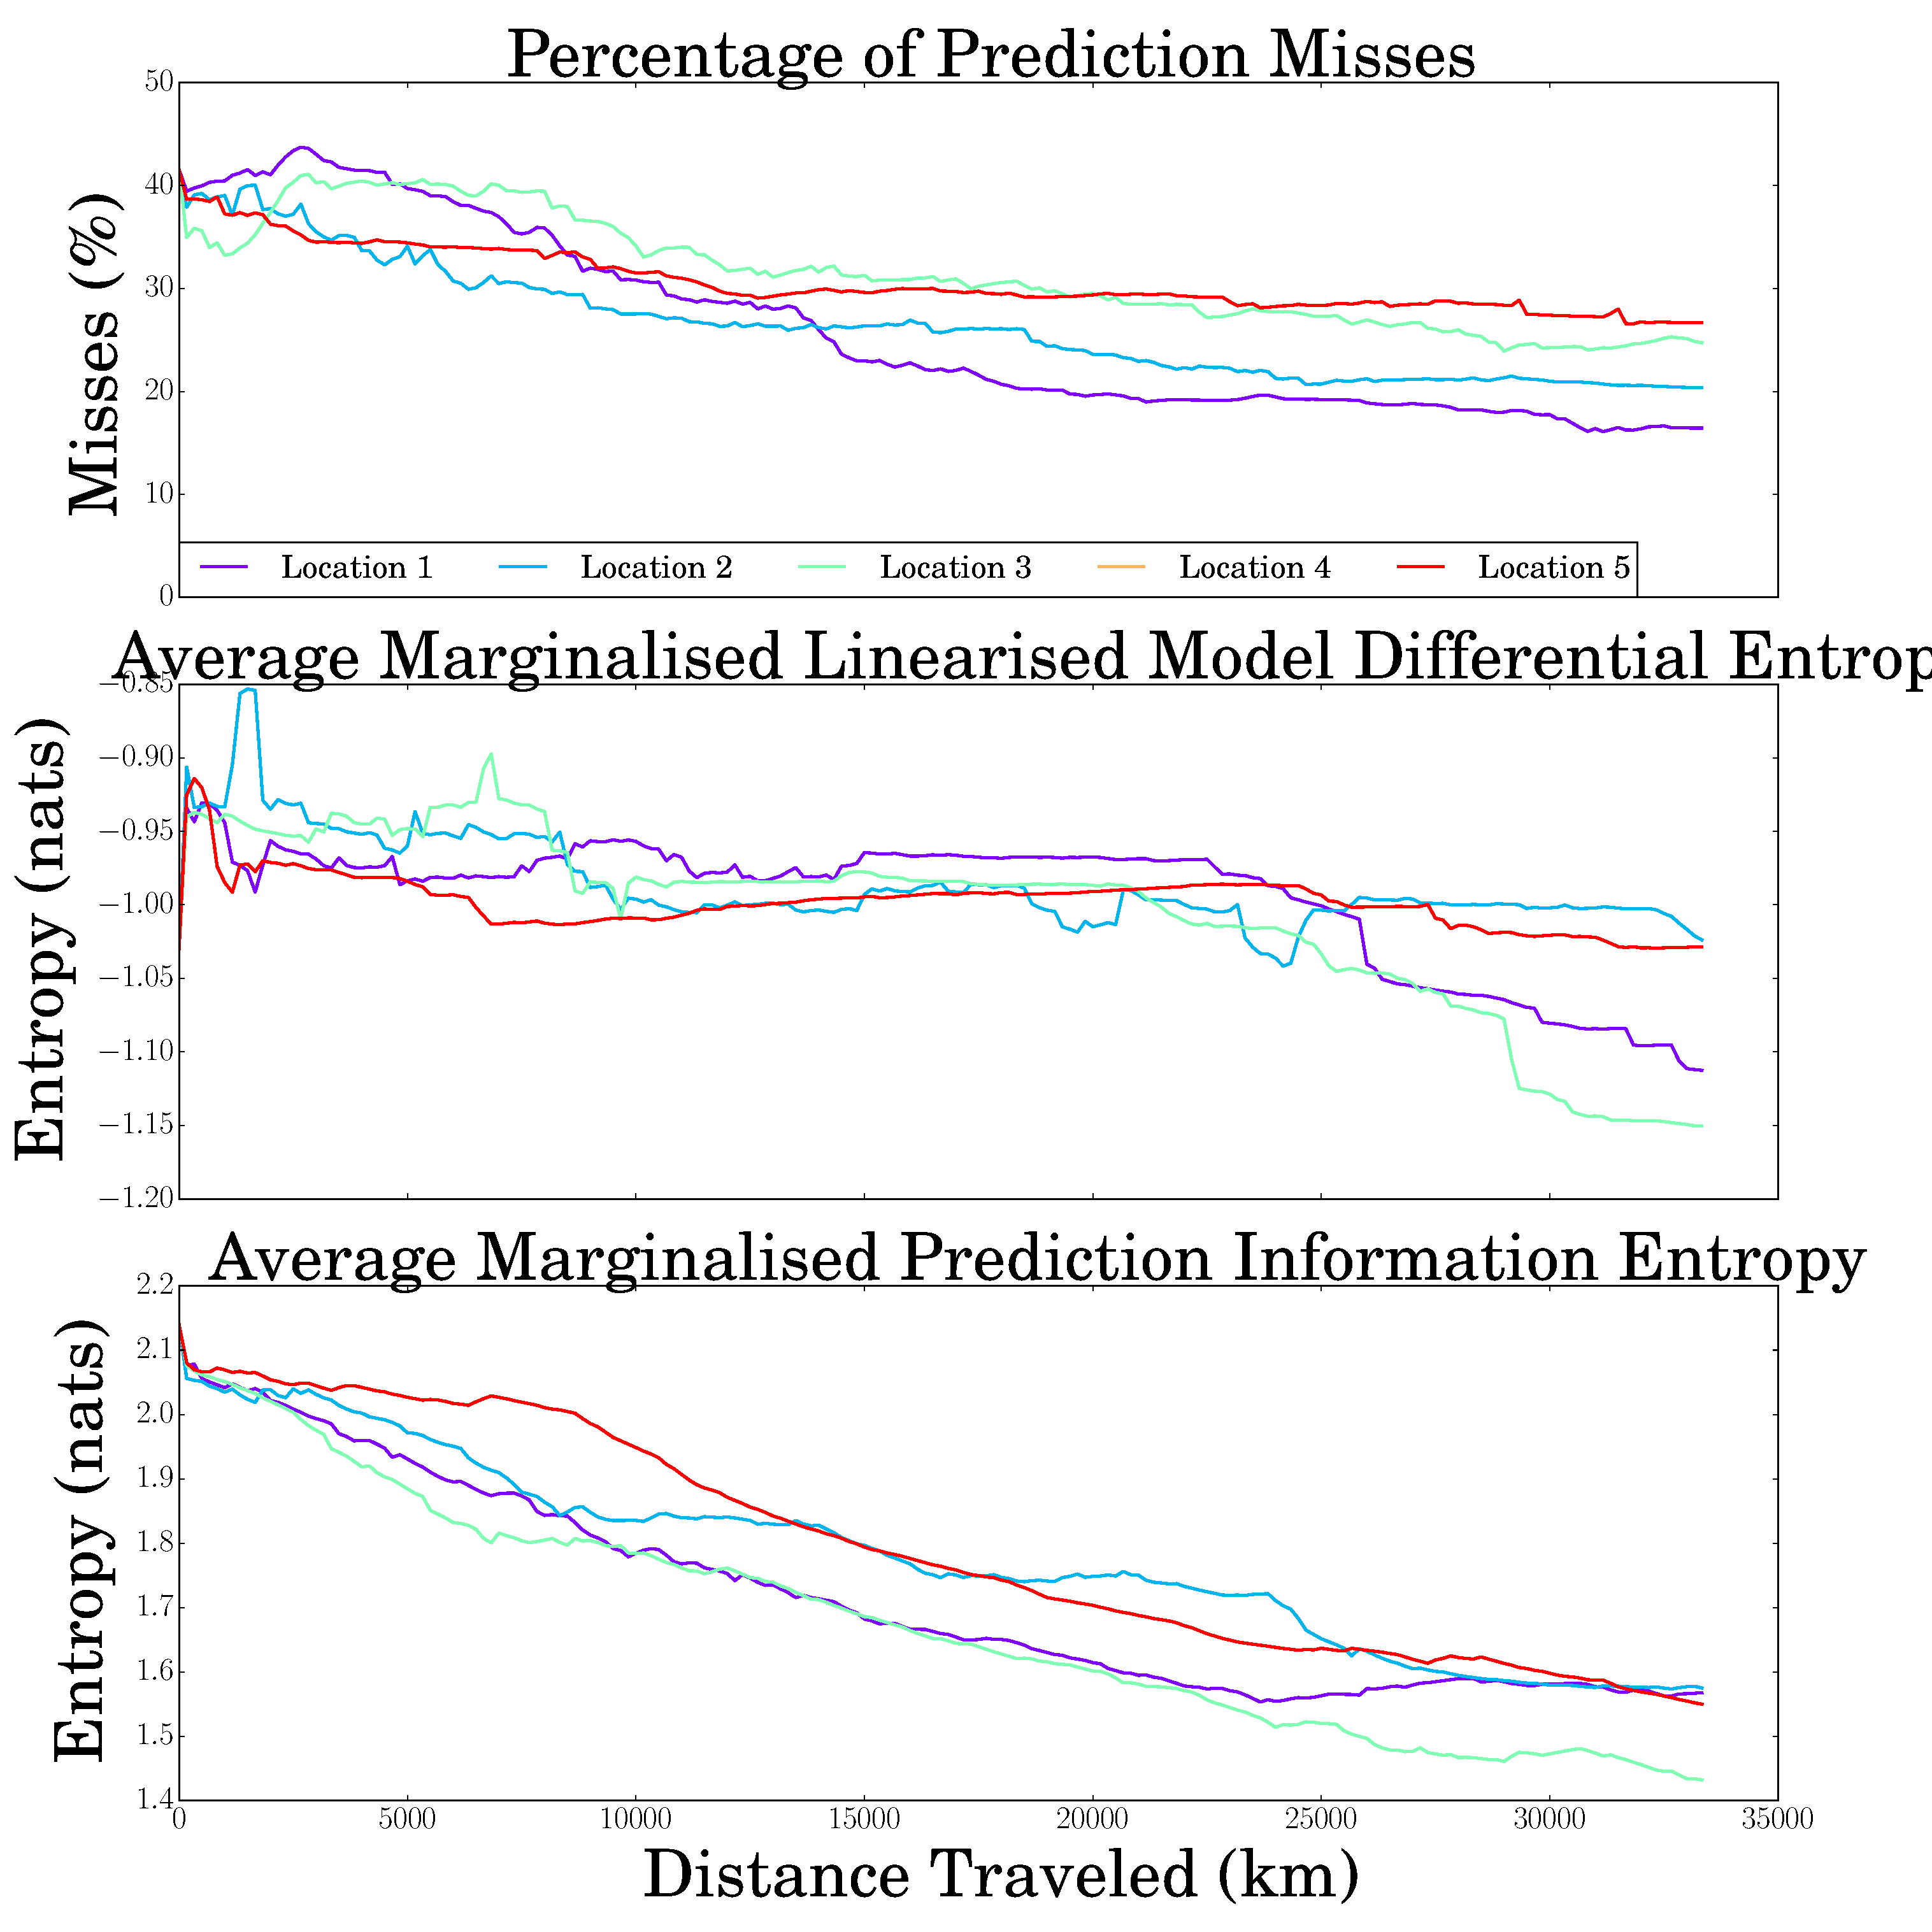
\includegraphics[width=0.48\linewidth]{Figures/compare_locations.eps}}
			  \subfigure[Receding Horizon Lengths]{\label{Figure:CompareHorizons}	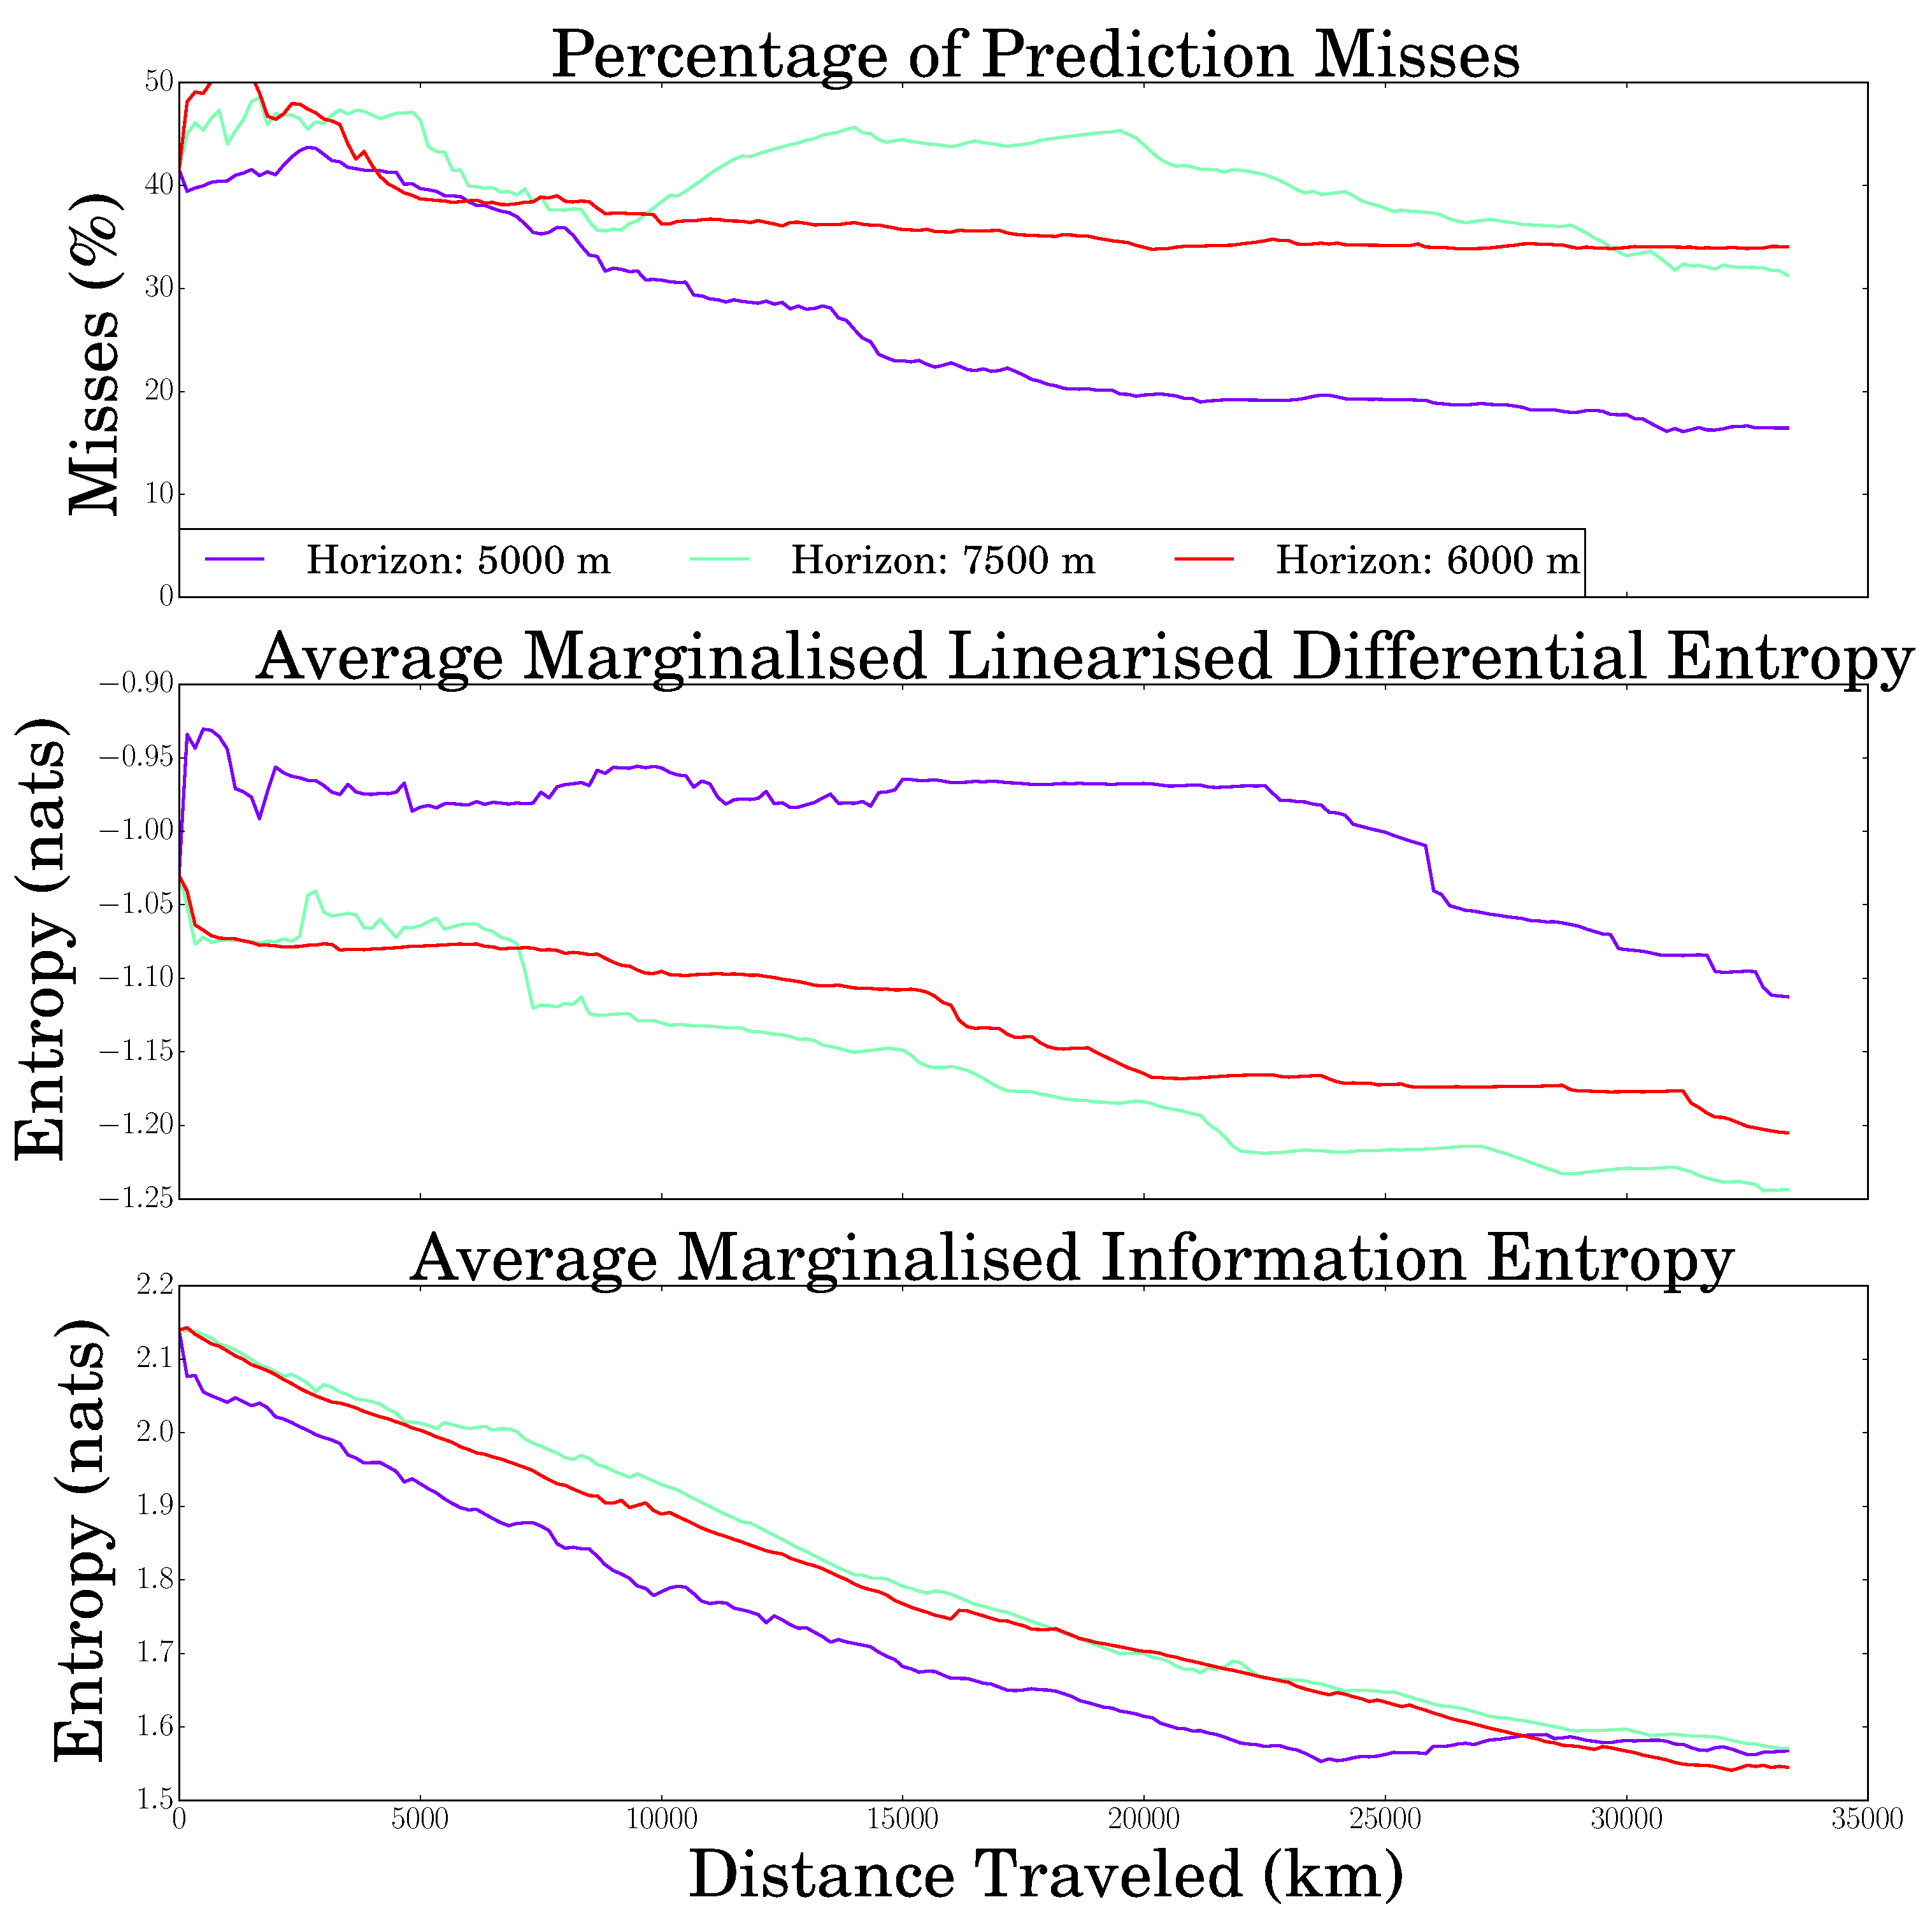
\includegraphics[width=0.48\linewidth]{Figures/compare_horizons.eps}}
			\caption{Variance across initial starting point and receding horizon lengths}
			\label{Figure:VarianceSimulation}
			\end{figure}	
				
			Figure \ref{Figure:VarianceSimulation} demonstrates the stability and consistency of the LMDE acquisition approach under varying horizon lengths and starting locations for the case of Scott Reef. 
			
	\section{Serial Mission Planning}
	\label{Appendix:SeafloorExplorationTimeLapse:Serial}
	
			Figures \ref{Figure:SerialOptimalPaths:PIE:LMDE} and \ref{Figure:SerialOptimalPaths:PIE:MCPIE} shows the prediction information entropy map for both LMDE acquisition and MCPIE acquisition under serial mission planning respectively for reference. Similar to the single mission planning case, it can be observed that the entropy of regions with similar bathymetric features are reduced together. This is again because the benthic habitats are modeled upon bathymetric features instead of the habitat locations, which allows inferences to be made between locations that are potentially faraway.
			
			\begin{figure}[!htbp]
			\centering
			  \subfigure[Journey: 1\%]{\label{Figure:SerialOptimalPaths:PIE:LMDE1} 
			  	\includegraphics[width = 0.31\linewidth]{Figures/informative_seafloor_exploration/serial_lmde/mie_propose1.eps}}
			  \subfigure[Journey: 5\%]{\label{Figure:SerialOptimalPaths:PIE:LMDE2} 
			  	\includegraphics[width = 0.31\linewidth]{Figures/informative_seafloor_exploration/serial_lmde/mie_propose10.eps}}
			  \subfigure[Journey: 25\%]{\label{Figure:SerialOptimalPaths:PIE:LMDE3} 
			  	\includegraphics[width = 0.31\linewidth]{Figures/informative_seafloor_exploration/serial_lmde/mie_propose50.eps}}
			  \subfigure[Journey: 50\%]{\label{Figure:SerialOptimalPaths:PIE:LMDE4} 
				\includegraphics[width = 0.31\linewidth]{Figures/informative_seafloor_exploration/serial_lmde/mie_propose100.eps}}
			  \subfigure[Journey: 75\%]{\label{Figure:SerialOptimalPaths:PIE:LMDE5} 
			  	\includegraphics[width = 0.31\linewidth]{Figures/informative_seafloor_exploration/serial_lmde/mie_propose150.eps}}
			  \subfigure[Journey: 100\%]{\label{Figure:SerialOptimalPaths:PIE:LMDE6} 
			  	\includegraphics[width = 0.31\linewidth]{Figures/informative_seafloor_exploration/serial_lmde/mie_propose199.eps}}
			\caption{Scott Reef: LMDE Acquisition}
			\label{Figure:SerialOptimalPaths:PIE:LMDE}
			\end{figure}
			
				
			\begin{figure}[!htbp]
			\centering
			  \subfigure[Journey: 1\%]{\label{Figure:SerialOptimalPaths:PIE:MCPIE1} 
			  	\includegraphics[width = 0.31\linewidth]{Figures/informative_seafloor_exploration/serial_lmde/mie_propose1.eps}}
			  \subfigure[Journey: 5\%]{\label{Figure:SerialOptimalPaths:PIE:MCPIE2} 
			  	\includegraphics[width = 0.31\linewidth]{Figures/informative_seafloor_exploration/serial_mcpie/mie_propose10.eps}}
			  \subfigure[Journey: 25\%]{\label{Figure:SerialOptimalPaths:PIE:MCPIE3} 
			  	\includegraphics[width = 0.31\linewidth]{Figures/informative_seafloor_exploration/serial_mcpie/mie_propose50.eps}}
			  \subfigure[Journey: 50\%]{\label{Figure:SerialOptimalPaths:PIE:MCPIE4} 
				\includegraphics[width = 0.31\linewidth]{Figures/informative_seafloor_exploration/serial_mcpie/mie_propose100.eps}}
			  \subfigure[Journey: 75\%]{\label{Figure:SerialOptimalPaths:PIE:MCPIE5} 
			  	\includegraphics[width = 0.31\linewidth]{Figures/informative_seafloor_exploration/serial_mcpie/mie_propose150.eps}}
			  \subfigure[Journey: 100\%]{\label{Figure:SerialOptimalPaths:PIE:MCPIE6} 
			  	\includegraphics[width = 0.31\linewidth]{Figures/informative_seafloor_exploration/serial_mcpie/mie_propose199.eps}}
			\caption{Scott Reef: MCPIE Acquisition}
			\label{Figure:SerialOptimalPaths:PIE:MCPIE}
			\end{figure}
			
			Figures \ref{Figure:SerialOptimalPaths:LMDE} and \ref{Figure:SerialOptimalPaths:MCPIE} show the prediction map of the exploration process for LMDE and MCPIE acquisition. Unlike the case before, since the exploration is initialised with only 17 observations, the prediction map changes drastically in the beginning, and slowly stabilises as exploration continues.

			\begin{figure}[!htbp]
			\centering
			  \subfigure[Journey: 1\%]{\label{Figure:SerialOptimalPaths:LMDE1} 
			  	\includegraphics[width = 0.31\linewidth]{Figures/informative_seafloor_exploration/serial_lmde/pred_propose1.eps}}
			  \subfigure[Journey: 5\%]{\label{Figure:SerialOptimalPaths:LMDE2} 
			  	\includegraphics[width = 0.31\linewidth]{Figures/informative_seafloor_exploration/serial_lmde/pred_propose10.eps}}
			  \subfigure[Journey: 25\%]{\label{Figure:SerialOptimalPaths:LMDE3} 
			  	\includegraphics[width = 0.31\linewidth]{Figures/informative_seafloor_exploration/serial_lmde/pred_propose50.eps}}
			  \subfigure[Journey: 50\%]{\label{Figure:SerialOptimalPaths:LMDE4} 
				\includegraphics[width = 0.31\linewidth]{Figures/informative_seafloor_exploration/serial_lmde/pred_propose100.eps}}
			  \subfigure[Journey: 75\%]{\label{Figure:SerialOptimalPaths:LMDE5} 
			  	\includegraphics[width = 0.31\linewidth]{Figures/informative_seafloor_exploration/serial_lmde/pred_propose150.eps}}
			  \subfigure[Journey: 100\%]{\label{Figure:SerialOptimalPaths:LMDE6} 
			  	\includegraphics[width = 0.31\linewidth]{Figures/informative_seafloor_exploration/serial_lmde/pred_propose199.eps}}
			\caption{Scott Reef: LMDE Acquisition}
			\label{Figure:SerialOptimalPaths:LMDE}
			\end{figure}
					
			\begin{figure}[!htbp]
			\centering
			  \subfigure[Journey: 1\%]{\label{Figure:SerialOptimalPaths:MCPIE1} 
			  	\includegraphics[width = 0.31\linewidth]{Figures/informative_seafloor_exploration/serial_lmde/pred_propose1.eps}}
			  \subfigure[Journey: 5\%]{\label{Figure:SerialOptimalPaths:MCPIE2} 
			  	\includegraphics[width = 0.31\linewidth]{Figures/informative_seafloor_exploration/serial_mcpie/pred_propose10.eps}}
			  \subfigure[Journey: 25\%]{\label{Figure:SerialOptimalPaths:MCPIE3} 
			  	\includegraphics[width = 0.31\linewidth]{Figures/informative_seafloor_exploration/serial_mcpie/pred_propose50.eps}}
			  \subfigure[Journey: 50\%]{\label{Figure:SerialOptimalPaths:MCPIE4} 
				\includegraphics[width = 0.31\linewidth]{Figures/informative_seafloor_exploration/serial_mcpie/pred_propose100.eps}}
			  \subfigure[Journey: 75\%]{\label{Figure:SerialOptimalPaths:MCPIE5} 
			  	\includegraphics[width = 0.31\linewidth]{Figures/informative_seafloor_exploration/serial_mcpie/pred_propose150.eps}}
			  \subfigure[Journey: 100\%]{\label{Figure:SerialOptimalPaths:MCPIE6} 
			  	\includegraphics[width = 0.31\linewidth]{Figures/informative_seafloor_exploration/serial_mcpie/pred_propose199.eps}}
			\caption{Scott Reef: MCPIE Acquisition}
			\label{Figure:SerialOptimalPaths:MCPIE}
			\end{figure}
			